\chapter{Accurate Bike Routing}\label{ch:routing}

\begin{Summary}[Bibliographical Notes]
This chapter is based on the following paper in which the author was the principal investigator:

\cite{matthes2023accurate} \fullcite{matthes2023accurate}
\end{Summary}

\section{Introduction}

The mobility behavior in urban environments is becoming increasingly intermodal. The trend is moving towards a multimodal mobility planning \cite{park_framework_2023}, where bike-sharing and bike routes also play a significant role. Understanding cyclists' behaviors, particularly their route choices, is crucial not only for calculating preferences for suitable cycling routes but also as a fundamental aspect of expanding cycling infrastructure and urban planning \cite{zielstra_comparative_2011, huber_modelling_2021}. Models that replicate cyclists' route choices provide immediate insights into where cycling infrastructure should receive high priority. Effective route selection is indispensable for bicycle navigation applications, but the challenge lies in the high individuality and context dependence of chosen paths \cite{dill_revisiting_2016, schleinitz_german_2017, misra_modeling_2018}, resulting in a multi-criteria optimization problem \cite{song_exploring_2014}. Route choices depend not only on road conditions but also on factors such as bicycle type and personal preferences, making it challenging to compute optimal routes for cyclists.

In the context of GLOSA applications, routing is linked to additional factors. It is essential not only for the cycling route to follow reasonable paths but also to accurately align with bicycle lanes for precise traffic light matching. The closer the route aligns with the bicycle lane, the better it serves distance estimation to the traffic light. Accounting for bends or obstacles on the way to the traffic light ensures accurate distance estimation, preventing the speed recommendation from deviating from the actual speed. Additionally, factors such as route incline and road conditions contribute not only to routing but also serve as crucial information sources for speed recommendations. Accurate and consistent meta-information is desirable in these cases and must be obtained from a routing foundation.

Commercial map providers provide highly accurate map material but currently have the drawback of limited openness and extensibility. Considerations about copyright, privacy, costs, and vendor lock-ins are also relevant for these map providers, rendering them unattractive for many services. Thus, OpenStreetMap has established itself as the most popular foundation for various acknowledged solutions, such as Openrouteservice\footnote{\url{https://openrouteservice.org/}}, Photon and Komoot\footnote{\url{https://photon.komoot.io/}}, and Mapbox\footnote{\url{https://wiki.openstreetmap.org/wiki/Mapbox}}. Apple Maps and Bing Maps also use OpenStreetMap wherever no commercial data providers are available\footnote{\url{https://wiki.openstreetmap.org/wiki/Apple}, \url{https://wiki.openstreetmap.org/wiki/Bing_Maps}}. 

Despite being a highly recognized map foundation, an ongoing issue is that OpenStreetMap's accuracy and consistency vary due to its Volunteered Geographical Information (VGI) concept \cite{wasserman_evaluating_2019, jacobs_openstreetmap_2020, vybornova_automated_2023}. As a result, bicycle routes generated with OpenStreetMap may not always achieve the desired accuracy. With a highly engaged user base and various company-level contributors, OpenStreetMap profits from frequent updates. However, similar to Wikipedia, not all contributions are of high quality. As a result, bike paths are not always captured as separate geometries from the road or tagged with the correct properties.

In this chapter, we introduce an open alternative for accurate bicycle routing. We propose methods to reuse bike infrastructure reference models (authoritative datasets) that are institutionally maintained and released under open-source licenses. An example is the "Digitales Radnetz Hamburg" (Digital Cycling Network Hamburg, DRN), specifically designed for cycling paths in Hamburg. Such models promise a significantly more accurate and consistent resolution of cycling paths, making them an attractive solution for a GLOSA app. Other municipalities provide such models as well \cite{englede_efficient_2013, brovelli_towards_2017}. 

However, infrastructure reference models face the challenge of lacking global coverage. In the case of DRN, it covers only the city of Hamburg, making routing across city borders challenging. Solutions need to be devised for integrating the dataset with routing profiles for cyclists, addressing various technical challenges. Given that both DRN and OpenStreetMap lack elevation data, selecting the best provider from several available elevation providers is crucial. The goal is to outline precise steps that can help utilize similar datasets for bicycle routing in other regions and develop an open routing engine applicable beyond the GLOSA app for accurate bicycle routing in Hamburg.

Apart from the methodological aspect, the core contribution primarily lies in the results section. A key focus is evaluating how much the accuracy of traffic light matching can be improved with a potentially more precise representation of cycling paths, compared to results from \Cref{ch:matching}. The primary contribution is determining the effectiveness of routing based on this type of dataset by comparing alignment with cycling infrastructure and the number of routing errors. Ideally, using the open DRN routing foundation should resolve many of the issues found with OpenStreetMap bike routing, providing users of the bike-GLOSA app with much better directions and speed recommendations.

\section{Related Work}\label{sec:rw-uis}

Establishing an accurate bike routing is a multifaceted research area. One avenue of investigation focuses on models that can predict cyclists' route choices with high accuracy based on available metadata \cite{dill_understanding_2008, ghanayim_modelling_2018, huber_modelling_2021}. This involves correlating GNSS trajectories with routing networks to understand the relationships between path characteristics and route selection \cite{sultan_extracting_2017, huber_modelling_2021}. Some studies also focus on safe bike routing \cite{loidl_online_2018}, popularity-based routing \cite{bergman_conflation_2016} or the short-term effects of infrastructure changes on cyclists' route preferences \cite{yeboah_route_2015, pritchard_does_2019}. Over the years, open routing engines such as GraphHopper\footnote{\url{https://www.graphhopper.com/}} have continuously improved, providing community and research-tested routing profiles tailored for various types of cycling. Thus, although there are optimization opportunities for bike routing profiles \cite{krismer_elevation_2016}, the available ones can be considered well consolidated.

Our focus will be on the issue of achieving a more accurate routing foundation and its application scenarios in GLOSA systems. First, we will discuss the status quo of bike path consistency and accuracy in routing foundations. Looking for solutions to the problem, we will investigate methods that utilize external authoritative datasets to improve the overall quality and alignment of bike path segments. Subsequently, we will delve into several challenges for GLOSA systems where precise routing emerges as a key solution. These challenges include multi-segment GLOSA, GNSS error correction, context-sensitive speed advisories, traffic light matching, and distance-to-signal estimation.

\subsection{Bike Path Consistency and Accuracy in Routing Foundations}

How accurately and consistently a bike routing can be performed depends on the specific kind of routing foundation: VGIs such as OpenStreetMap, commercial providers such as Google Maps and Bing Maps, or authoritative infrastructure datasets.

A first finding is that the commercial providers Google Maps and Bing Maps do not necessarily provide a more consistent and accurate depiction than OpenStreetMap. Ciepluch's comparison in 2010 \cite{ciepluch_comparison_2010} revealed that Google Maps, Bing Maps, and OpenStreetMap did not significantly differ in quality, with no platform emerging as a clear winner. Similarly, a more recent study by Franzini et al. (2020) \cite{franzini_assessment_2020} found that only 40\% of the Pavia region in Italy is fully mapped in OpenStreetMap and 30\% in Google Maps, based on 2018 data. This study is not specifically focused on bicycle paths.

Hochmair et al. (2015) \cite{hochmair_assessing_2015}  specifically assessed the coverage of bicycle infrastructure, noting variations in completeness. In Portland, 86.4\% of 26 km of bicycle trails were correctly captured in OpenStreetMap, compared to 78.4\% in Google Maps. However, in Miami, only 22.8\% (OpenStreetMap) and 36.5\% (Google Maps) of 22 km of reference paths were accurately recorded, with a significant omission of paths along recreational sites such as rivers and parks. 

Additionally, Ferster et al. (2019) \cite{ferster_using_2019} and Wasserman et al. (2019) \cite{wasserman_evaluating_2019} highlighted inconsistencies in meta-information about bike path quality in OpenStreetMap, impacting the determination of bikeability. Vybornova et al. (2023) \cite{vybornova_automated_2023} demonstrated that connectivity issues in bicycle path segments could disrupt meaningful route calculations, collectively indicating deficiencies in the coverage of bicycle infrastructure by OpenStreetMap and alternatives like Google Maps.

Identifying errors in OpenStreetMap data is relatively well investigated. Authoritative datasets have been used as ground truths for comparison, as demonstrated by various studies \cite{haklay_how_2010, jokar_arsanjani_quality_2015, ludwig_comparison_2011}. Brovelli et al. (2017) \cite{brovelli_towards_2017} introduced a framework for comparing open reference map data with OpenStreetMap, focusing on enhanced reusability. 

However, the question remains how the detected issues can be systematically resolved. Vybornova et al. (2023) \cite{vybornova_automated_2023} recently suggested a method to detect and rectify missing connections between bike paths, though this approach does not address missing meta-information or entirely absent bike paths. Nasiri et al. (2018) \cite{nasiri_improving_2018} introduced a multi-stage approach in which outliers are detected in OpenStreetMap histories, improving the positional precision of features by 14\% in Teheran.  

Some studies explore connecting meta-information from an authoritative reference model to OpenStreetMap for a more consistent metadata coverage, utilizing map-matching directly or methods that resemble established map-matching approaches \cite{chao_survey_2020}. Szwoch (2018) \cite{szwoch_combining_2019} demonstrated the integration of OpenStreetMap routes with metadata from an authoritative database. Fan et al. (2016) \cite{fan_polygon-based_2016} examined a similar approach. Meister et al. (2023) \cite{meister_route_2023} studied cyclists' route choices in Zurich, using map-matching to incorporate metadata from a municipal dataset due to OpenStreetMap's insufficient consistency. All three approaches address the issue of inconsistent metadata but not the issue of inaccurate route geometries as a result of missing or imprecise routing network geometries.

Building on these ideas, Smarzaro et al. (2021) \cite{smarzaro_creation_2021} demonstrate how data from multiple authoritative datasets and VGIs can be fused for improved multimodal routing. The focus is on uncovering unknown paths, such as footpaths in parks or parking lots, and associated meta-information. The authors propose a method where each geospatial feature from an external dataset is compared to nearby paths, and if new, it is added to the dataset. However, the challenge lies in defining suitable thresholds to distinguish overlapping from non-overlapping segments. The study, unfortunately, only compares travel distances with Google Maps without a thorough assessment of improved coverage or accuracy. Whether bike paths are captured separately to nearby segments and, thus, how the alignment with individual lanes on intersection topologies is affected by such an approach is also an open question.

Li et al. (2017) \cite{li_optimized_2017} demonstrate how OpenStreetMap can be inserted into an authoritative bikeway dataset to enhance the overall accuracy of bikeway geometries and metadata. The authors employ a semi-automated approach with a human-in-the-loop that performs four steps: first, the datasets are preprocessed to ensure their consistency and correct geographical projection. Afterward, the datasets are automatically conflated, including metadata mapping to match OpenStreetMap path tags to four path categories in their authoritative dataset. In the third and fourth steps, the quality of paths is evaluated using the feature matching uncertainty and a human eye, allowing a human to manually adjust false matchings. In their evaluation, the authors found their system to achieve a relatively high precision of 92.54\%. 

Here, it needs to be considered that the authors conducted their study on a relatively sparse bike path dataset in Los Angeles. Thus, one main limitation the authors noted is the reliance on human intervention with false matchings. A fully automated approach would be desirable to account for the continuously evolving bike infrastructure without having to conduct a manual correction process on a daily basis. Furthermore, the authors claim to have improved positional accuracy of the bike path geometries. However, no concrete measures w.r.t to a ground truth are presented. Further investigations are required to address these limitations.

In summary, the inaccuracy and inconsistency of OpenStreetMap is a relatively well-known issue. Approaches to solve this problem focus on combining OpenStreetMap with authoritative datasets. Two approaches by Smarzaro et al. (2021) \cite{smarzaro_creation_2021} and Li et al. (2017) \cite{li_optimized_2017} also aim to correct geometrical information in the path network, not only its metadata. However, the main limitation of these approaches is an overall limited investigation of the effects of correction on the alignment accuracy with actual infrastructure, i.e., a ground truth such as lane geometries. Both approaches focus on unifying individual path segments, trading off with the need to decide or average between matching path segments. Replacing entire areas in OpenStreetMap with covered proportions of a reference dataset, assuming the reference dataset is closer to the ground truth, is another opportunity since it could drastically reduce the chances for individual mismatches and thus increase automation. This idea, however, shifts the problem of dataset harmonization towards stitching in boundary regions, requiring further attention.

\subsection{Application Scenarios of Routing in GLOSA}

- Multi-segment GLOSA

- GNSS Error Correction

- Metadaten für Kontextsensitivität und Routing-Profile

- Traffic light matching

- Distance-to-signal estimation

\section{Concept}

\subsection{DRN Routing}

Routing with GraphHopper and OpenStreetMap has the advantages of worldwide support and frequent updates of the community. However, the quality and consistency of the map materials vary from location to location. Since OpenStreetMap is a general-purpose map foundation, bike paths are often not represented as separate geometries but instead merged with the nearby road. This leads to the problem that some roads have separate bike path geometries running alongside, and others don't. Hence, when calculating a bike route based on OpenStreetMap, the bike route often jumps on or off the road. This degrades the distance-to-signal estimation, traffic light matching, and overall in-app routing. Although the system may work with OpenStreetMap, this situation is still not ideal.

To counteract this problem, it is vital to look for other routing foundations than OpenStreetMap that model the bike paths more accurately. As a solution, the dataset "Digitales Radverkehrsnetz Hamburg"\footnote{\url{https://metaver.de/trefferanzeige?docuuid=EA847D9F-6403-4B75-BCDB-73F831F960C7}} (DRN) has been identified. The dataset is institutionally maintained and contains all bikeable paths in Hamburg. Based on preliminary comparisons with OpenStreetMap, the DRN dataset promises a more consistent and quality-assured depiction of bike paths.

\begin{figure}[htbp]
\centering
\begin{subfigure}
  \centering
  
\includegraphics[width=\linewidth]{images/legend-fig-1.png}
\end{subfigure}
\begin{subfigure}
  \centering
  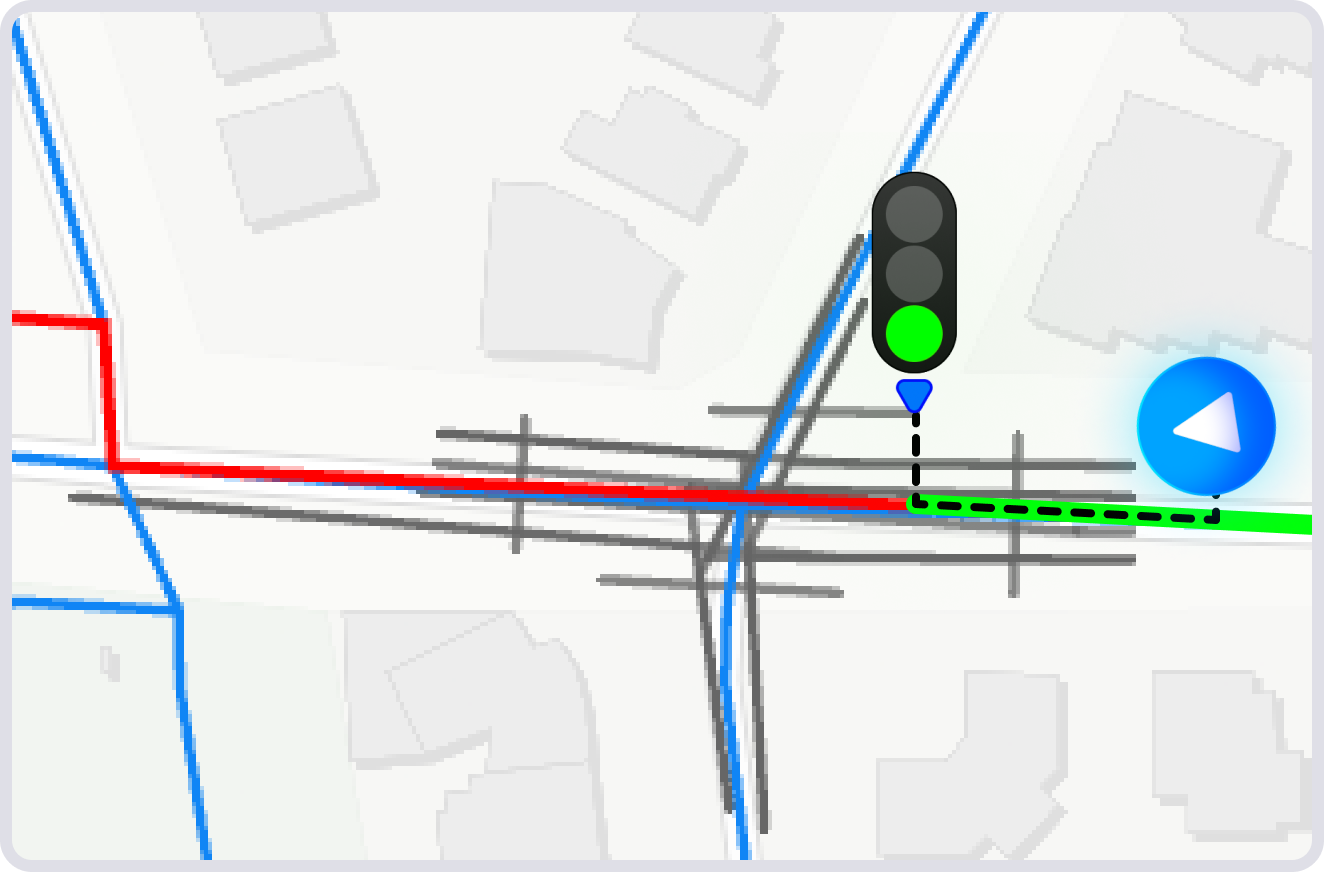
\includegraphics[width=.49\linewidth]{images/osm-route.png}
\end{subfigure}%
\begin{subfigure}
  \centering
  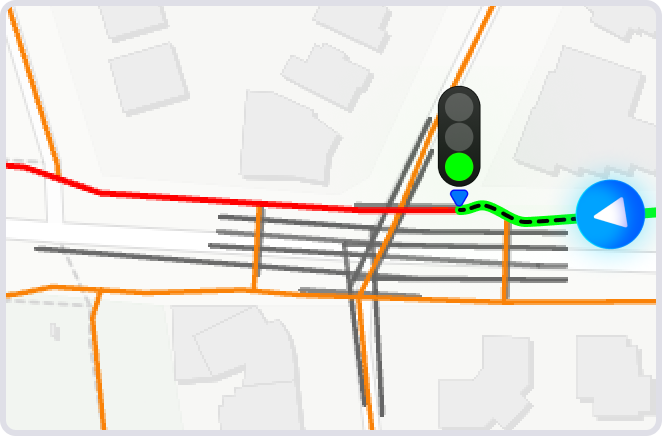
\includegraphics[width=.49\linewidth]{images/drn-route.png}
\end{subfigure}
\caption{Alignment of OpenStreetMap vs. DRN with the intersection topology. Image source: [in print].}
\label{fig:comparison}%
\end{figure}

\Cref{fig:comparison} shows a specific example of OpenStreetMap routing on the road when no separate bike path geometry is captured. With DRN the bike path is not only captured as a separate geometry but also aligns more closely with the bike path's curvature. Thus, the speed advisory could also be more precise as the signal's distance may be estimated more accurately. \Cref{fig:comparison} also highlights that the DRN route may align more closely with the bike signal's geometry, while the OpenStreetMap route is closer to the car lanes. Assuming that a cyclist follows the designated bike path, less speculation is required as to which traffic light must be matched. 

Due to these prospects, a system was created that allows for DRN-based bike routing inside Hamburg and OpenStreetMap-based bike routing outside Hamburg. To make DRN ready for routing, several processing steps were established as part of a publication at ITSC 2023 [in print], based on the supervised Diploma thesis of Max Lorenz (2022) \cite{lorenz_2022}: First, the DRN format must be translated into a data format that a routing engine understands. Then, the map's topology must be optimized such that routing errors are minimized. Finally, OpenStreetMap and DRN must be merged together at the city's border to allow a seamless transition.

\subsubsection{Translation from DRN to OpenStreetMap}

\begin{figure}[htbp]
\centering
\includegraphics[width=\linewidth]{images/drn-map.png}
\caption{An overview of the DRN dataset and its top-10 bike path types.}
\label{fig:drn-map}
\end{figure}

The DRN dataset can be downloaded in various geodata formats such as CSV, GeoJSON, or GML. Each contained data point refers to a path segment and is associated with metadata tags. Among others, the following properties are mapped\footnote{The displayed statistics represent a snapshot of the 23rd of August 2023.}:

\begin{itemize}
    \item Direction of travel (49852 segments bidirectional and 47692 segments unidirectional)
    \item Time restrictions (32 segments affected)
    \item Temporary paths such as pop-up lanes or detours (83 segments affected)
    \item If a segment is associated with a specific velo route or designated bike tours (Freizeitroute)
    \item Level (96237 flat, 1121 across bridges, 186 through tunnels)
    \item Obstacles (456 impassable, 52 can be circumvented e.g. via footpath)
    \item The type of bike path and its surface
    \item Target and end node ID of the segment connecting the segments to a graph
    \item The segment's coordinates
\end{itemize}

Now, to calculate routes based on the dataset, it is necessary to make the dataset available to the routing engine. Here, it is possible to design a plugin for the routing engine that allows it to read the dataset's format. However, a better solution is to transform the DRN dataset into the OpenStreetMap format. In this way, the existing routing engine and its community-tested routing profiles can be reused without modifying the engine's internals. Furthermore, transforming the DRN dataset to OpenStreetMap simplifies merging both datasets together at the city border. Thus, a map transformer was designed in [in print] that converts the DRN format to OpenStreetMap.

The routing profiles utilize weights of the properties annotated to each OpenStreetMap path to calculate a personalized route. The challenge here is that DRN specifies other properties than OpenStreetMap. For example, DRN specifies three types for compacted surface: "befestigt - nicht genauer erkennbar", "befestigt - zu detailieren" and "Wassergebundene Decke". To resolve this problem, a mapping was developed that infers the OpenStreetMap tags from the DRN specification. This mapping includes the bike path's surface, level, direction, and type (as shown in \Cref{fig:drn-map}). In cases where the bike path's properties cannot be directly mapped to a suitable OpenStreetMap tag, the path is tagged with \texttt{highway = tertiary}. As noted in [in print], this follows established mapping practices in Germany. The result is an inferred set of tags for each path in the OpenStreetMap format.

\subsubsection{Error Correction Methods}

After the map conversion into the OpenStreetMap format, there are still some problems with the map material that must be addressed. In [in print] two problems were identified when generating routes with the converted DRN network: detours resulting from duplicated nodes in the graph and detours because the road cannot be crossed.

\begin{figure}[htbp]
\centering
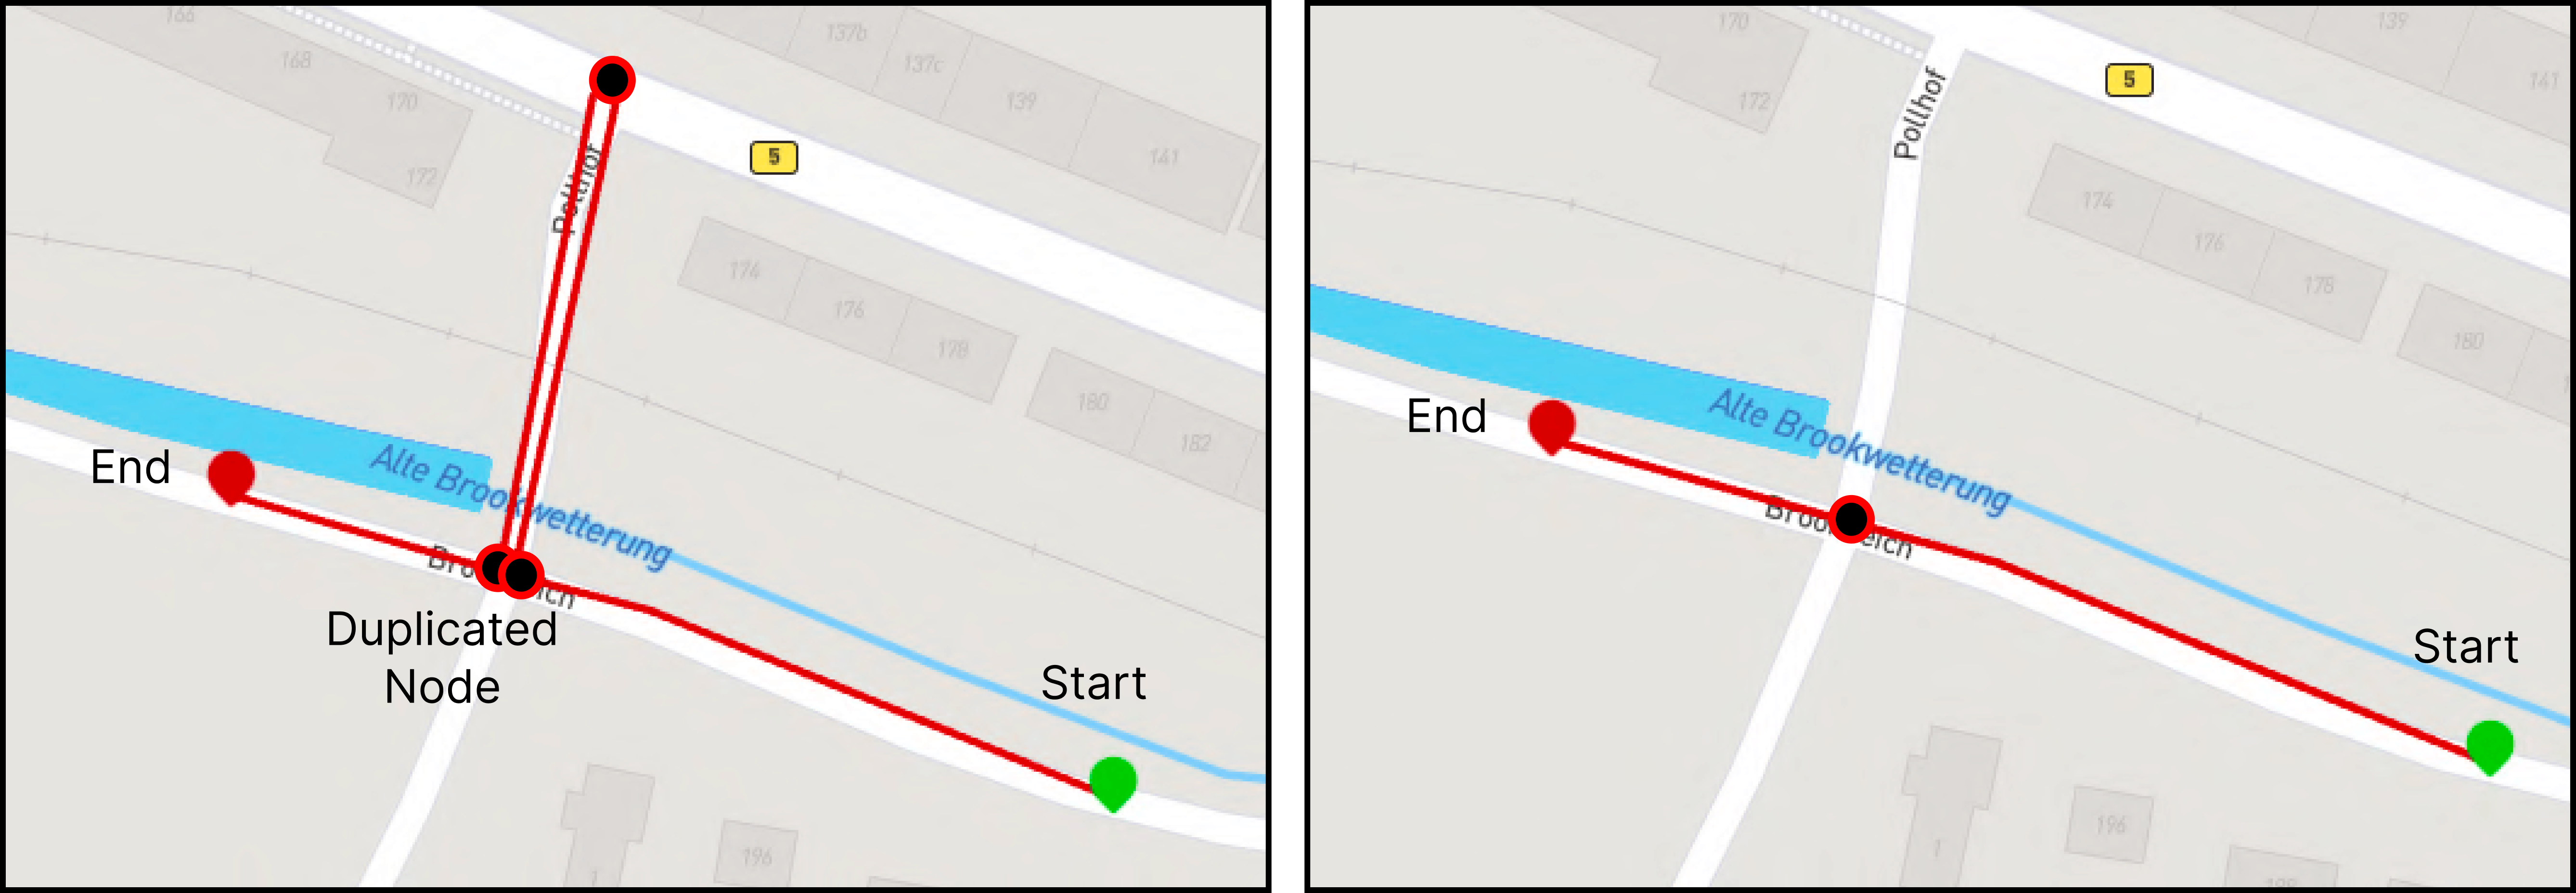
\includegraphics[width=\linewidth]{images/node-merging.png}
\caption{Duplicated nodes (left) are merged together (right) to avoid detours. Source: [in print]}
\label{fig:node-merging}
\end{figure}

\paragraph{Duplicated nodes:} Each individual path in the DRN dataset starts and ends in a node, which must be transformed into OpenStreetMap nodes that connect the individual paths to a graph structure\footnote{\url{https://wiki.openstreetmap.org/wiki/Node}}. To ease this process the DRN dataset provides node IDs for the start and end point of each path. Thus, two nodes are generated for each path based on the start and end coordinates given in the line geometry. Since there may be multiple paths that are connected to a node, the same node is generated multiple times during dataset processing. In theory, this is not a problem since the node ID can be utilized to avoid duplicates. In practice, however, sometimes there are nodes for which multiple different coordinates are found in the dataset. Due to presumably floating point or geographic projection inaccuracies in the dataset, the coordinates may be misaligned by a few centimeters.

As discussed in [in print], the developed solution involves calculating a center point for each node ID. Let $C_k = \{c_{k_1} = (lat_{k_1}, lng_{k_1}), \text{...} , c_{k_n} = (lat_{k_n}, lng_{k_n})\}$ be the collected coordinates for each node $k$. Then, the center point $\text{Center}_{\text{k}}$ is calculated as $\text{Center}_{\text{k}} = \left(n^{-1} * {\sum_{i=1}^{n} \text{{lat}}_{k_i}}, {n^{-1} * \sum_{i=1}^{n} \text{{lng}}_{k_i}}\right)$. The resulting coordinates are utilized to connect the generated paths. To validate this approach, the maximum relocation distance between all $\text{Center}_{\text{k}}$ and $c \in C_k$ was calculated as 8.3 centimeters using the haversine formula. Based on this result, no further points were falsely connected.

\paragraph{Non-crossable roads}: Since bike paths on both roadsides are captured as individual geometries in the DRN dataset, there may be long road segments with bike paths running in parallel. However, without interconnections between the roadsides, there is also no possibility for the route to cross the road. Sometimes, this represents a problem since side roads attached to the opposite roadside can only be reached by long detours. With OpenStreetMap, this is a lesser problem since roads are often captured as single-path geometries without a clear distinction between each roadside. 


\begin{figure}[htbp]
\centering
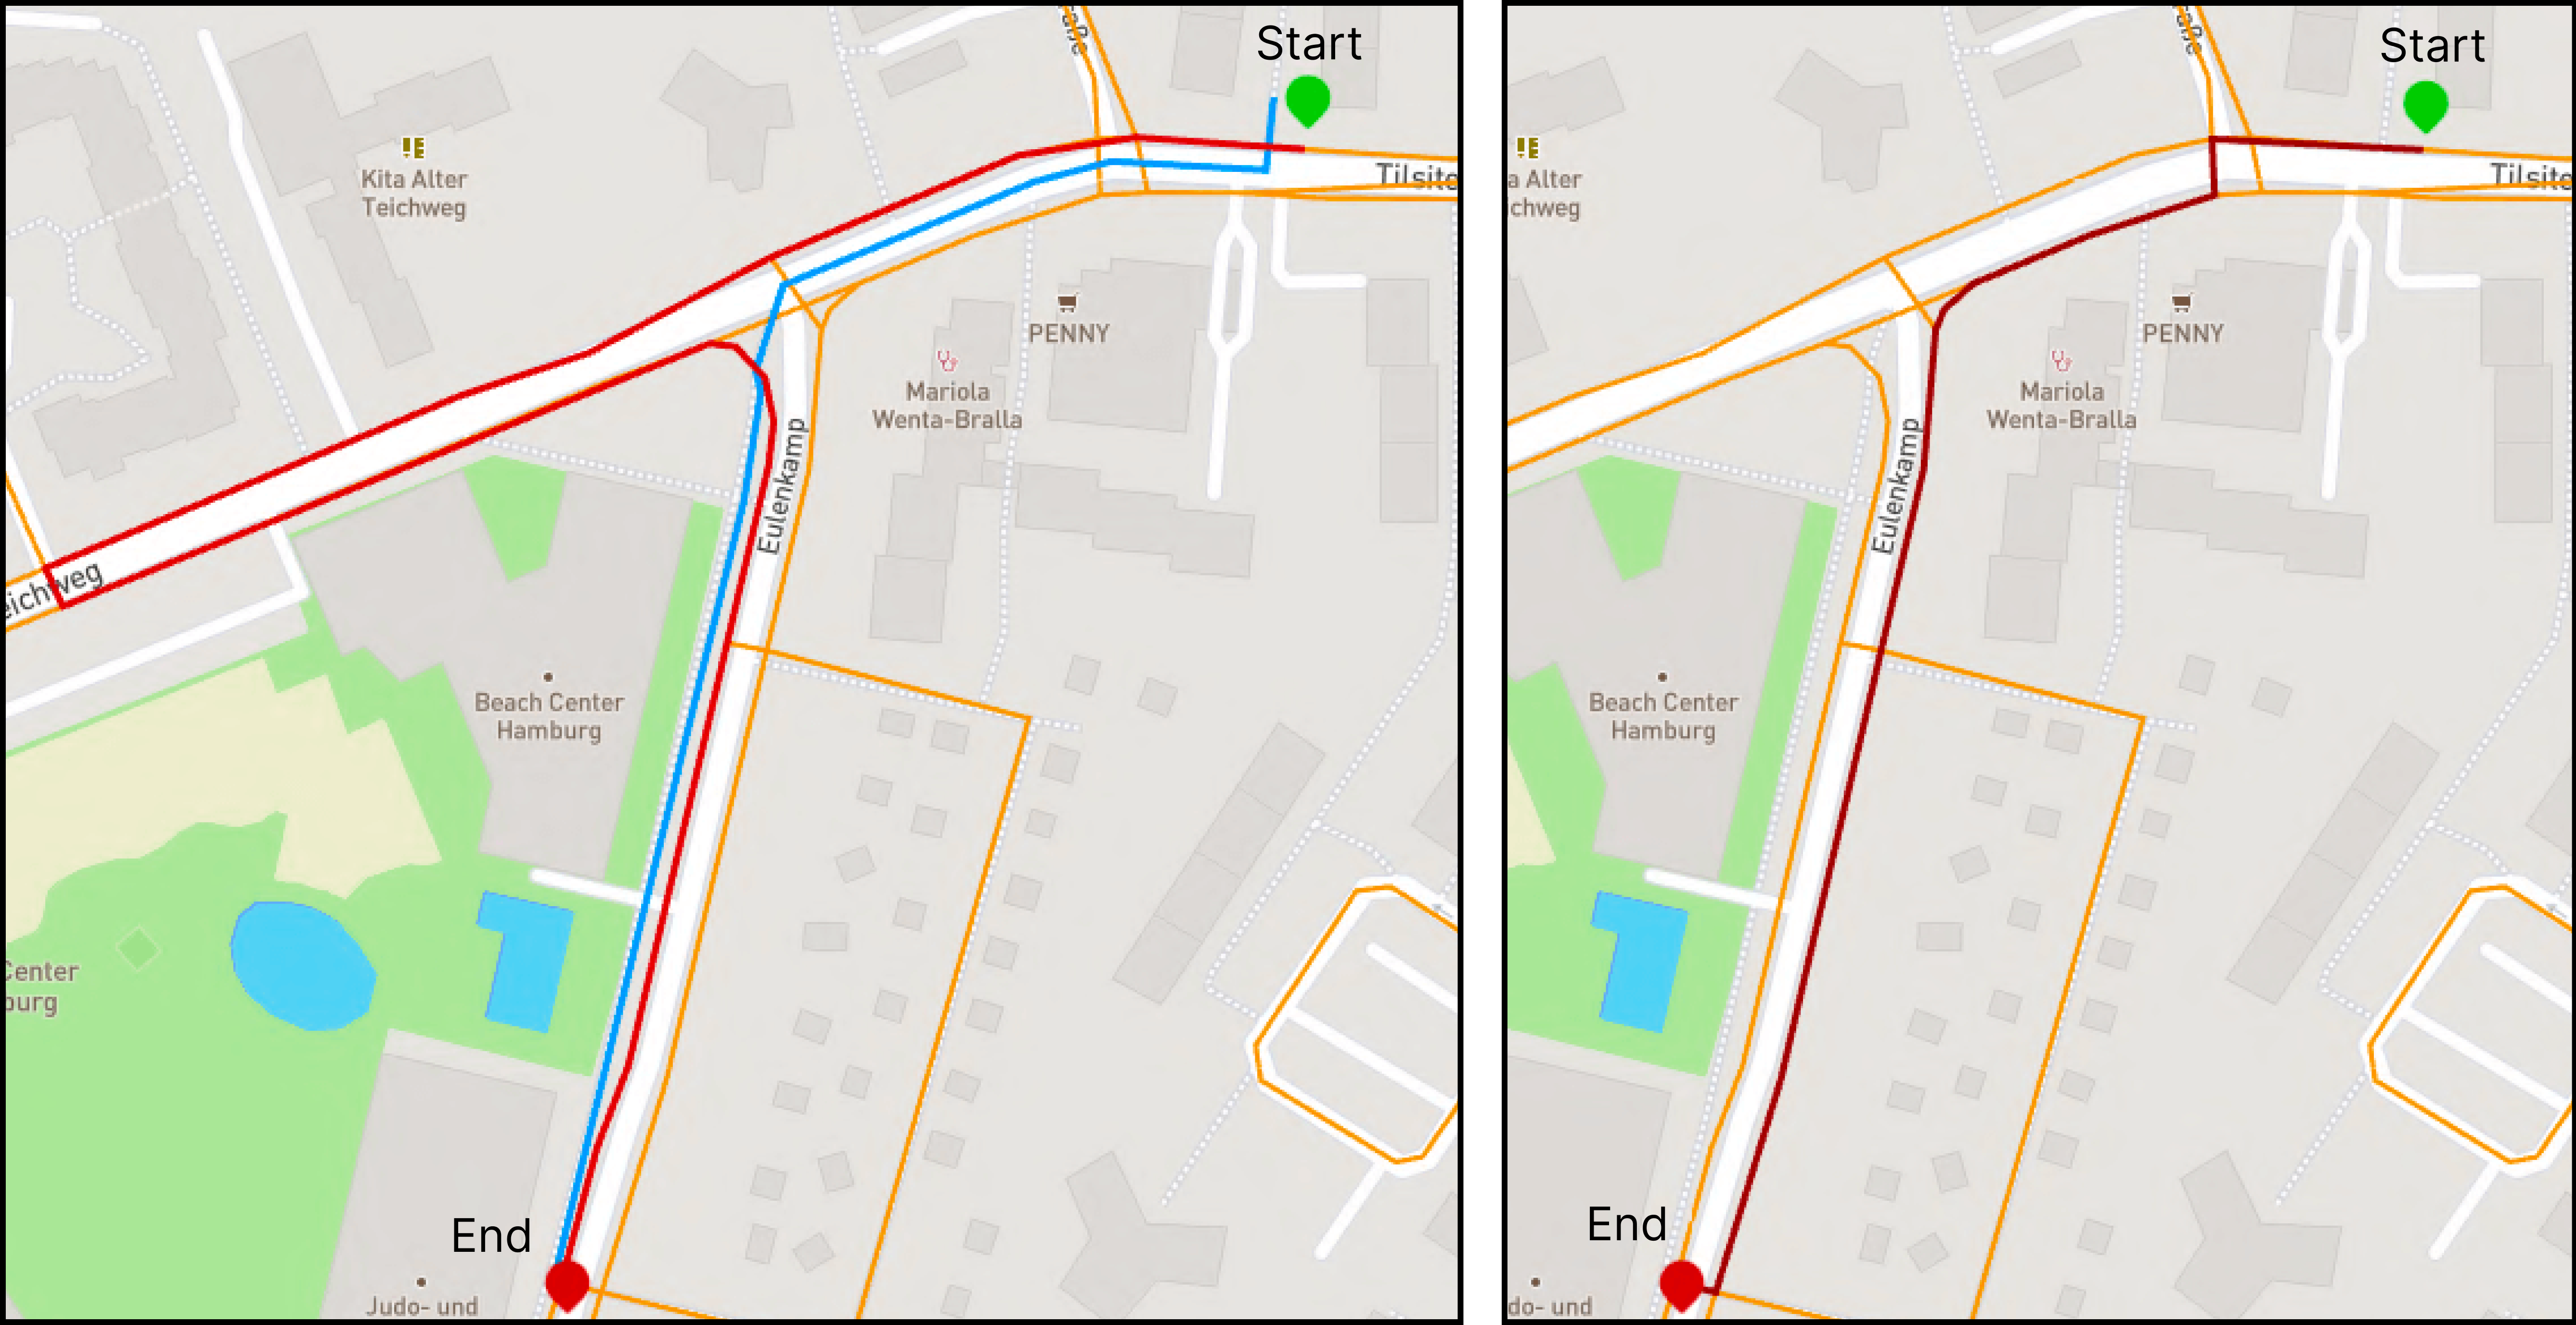
\includegraphics[width=\linewidth]{images/oneway-travel-fix.png}
\caption{Detour (left) that can be fixed by enabling opposite-direction one-way travel on foot (right), compared to OpenStreetMap route (blue). Source: [in print]}
\label{fig:oneway-travel-fix}
\end{figure}

One solution explored in [in print] is the introduction of "virtual" paths connecting the roadsides. Using these paths, the route could traverse between roadsides and avoid detours. Although this concept may sound like a reasonable idea at first, the question is where to place these virtual paths. For example, one could place these paths in a fixed interval along a road between roadsides. However, there could always be a physical barrier between both roadsides, meaning that generated routes would guide users over impassable obstacles or potentially encourage dangerous maneuvers. Traversing a road at an arbitrary location may not always be safe or legal. Due to these reasons, the idea of inserting virtual paths was discarded.

As discussed in [in print], the final solution takes another approach. In the DRN dataset, bike paths are marked for travel in one direction or two directions. Here, the error source for detours is often the restricted one-way travel direction along the bike path. In cases where detours are observed due to long paths down the street until the next road crossing, it is likely that a similar road crossing lies closer up the street. Thus, a solution is to allow opposite-direction one-way travel on foot. This solution assumes that the bike can safely and legally be dismounted and walked in the opposite direction.

\subsubsection{Routing Outside of Hamburg}

The DRN dataset's coverage ends at Hamburg's city border. This means that, although the dataset provides full coverage within the region of Hamburg, the dataset must be combined with another map foundation to provide routing outside the city. Here, it is possible to fall back to the OpenStreetMap dataset. However, the geometries of both datasets don't align. To provide continuous routing over the city border, both datasets must be stitched together. 

The conflation process presented in [in print] starts with matching the OpenStreetMap paths to the associated DRN paths along the city border. First, DRN nodes close (<20m) to the border are fetched. For each of these DRN nodes, the 5 nearest OpenStreetMap paths are treated as a possible match. However, the OpenStreetMap paths may traverse the city border without a node lying exactly on the border geometry, potentially leading to z-shaped connections between OpenStreetMap and DRN. To avoid this problem, the conflation process inserts artificial OpenStreetMap nodes at the intersection of the city border geometry. Finally, for each DRN node, the nearest (interpolated) OpenStreetMap node is selected and connected. As a result, the DRN paths are stitched to the OpenStreetMap paths along the city border.

Finally, the error-corrected and stitched path network is exported in the OpenStreetMap format. The exported map data is integrated with GraphHopper and replaces the original OpenStreetMap-only GraphHopper routing engine utilized by the mobile application.

\subsection{Digital Elevation Model}

With the chosen concept, users can personalize the routing algorithm to avoid inclines. In Hamburg, this may be less of a concern, but there are still several roads with non-negligible inclines such as Helgoländer Allee. However, DRN and OpenStreetMap don't directly include height data of the road network. Thus, without an external digital elevation model, the routing engine cannot consider paths accordingly using the specified routing profile. Fortunately, GraphHopper has a built-in option for integrating a digital elevation model.

As briefly discussed in [in print], there are multiple digital elevation models that can be used. By default, GraphHopper supports SRTM (Shuttle Radar Topography Mission) \cite{farr_shuttle_2000, farr_shuttle_2007} and CGIAR \cite{jarvis_hole_2008} height data. The CGIAR height data is a proprietary post-processed version of the SRTM data, filling in data gaps in the SRTM height map, and is available under license to all GraphHopper users. By default, the routing engine is specified to use the SRTM dataset.

SRTM-1 offers a horizontal resolution of approximately 30m (1 arcsecond). For specific areas, additional SRTM X-SAR 25m data is provided by the DLR. For the covered regions of the SRTM X-SAR 25m model, the vertical precision is specified at $\pm$ 6m (relative vertical error at 90\% confidence level)\footnote{SRTM X-SAR 25m specification: \url{https://geoservice.dlr.de/web/dataguide/srtm/}}. An even higher precision is offered by the DGM-1 model for Hamburg in which the 1 stands for 1 meter of horizontal resolution. In this model, the vertical resolution is specified as $\pm$ 15cm\footnote{\url{https://metaver.de/trefferanzeige?docuuid=A39B4E86-15E2-4BF7-BA82-66F9913D5640}}. The high precision is reached by airborne laser scanning. Downscaled resolutions are available as DGM-10 (10m) and DGM-25 (25m).

To evaluate if the DGM models provide an overall better height profile than SRTM, Max Lorenz analyzed cross-sections of the height models. Another important question of this work was how much resources the model consumes when loaded into the routing engine. The results, which have briefly been referenced in [in print], show that the best tradeoff between resource usage and model accuracy is provided by the DGM-10 model. Thus, the DGM-10 model was integrated as the final digital elevation model into the GraphHopper routing engine using a custom tileset download and parsing plugin. The result is a GraphHopper routing engine that not only runs on the DRN dataset but also utilizes the DGM-10 model to provide accurate, personalized routing while consuming an acceptable amount of resources. 

\subsection{Summary of Methods for Routing}

To summarize, an end-to-end routing solution was developed and fine-tuned to the needs of a bike-GLOSA application. Providing route personalization is an integral part of the application design. In this context, a user interface was designed that maps user-defined preferences to specific routing profiles for the routing engine. With additional visualizations of route metadata or the current traffic situation, users can plan their route accordingly. Geocoding and the visualization of points of interest help users find specific locations on the map. To fulfill the high accuracy demands for routing, a more accurate bike routing foundation based on DRN is integrated. Finally, a digital elevation model is incorporated to allow for incline-avoiding routing profiles.

\section{Results}

\subsection{Alignment with Actual Cycling Infrastructure}

\begin{figure}[htbp]
\centering 
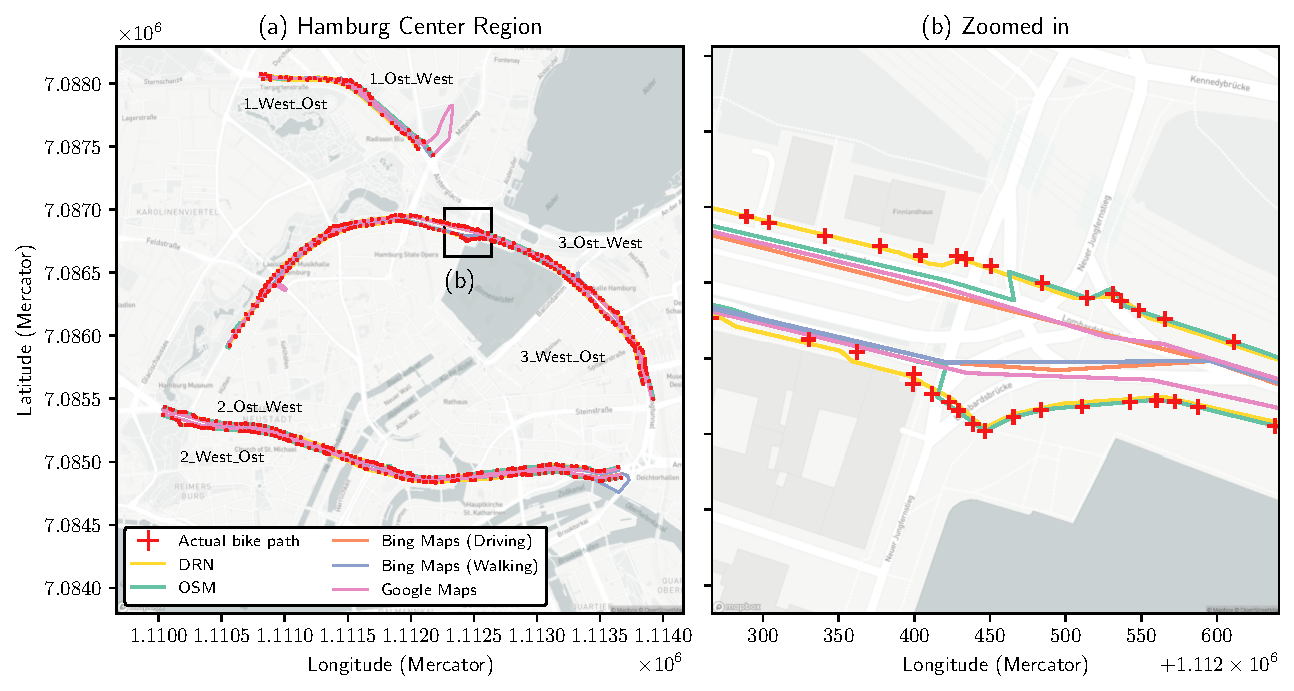
\includegraphics[width=\linewidth]{images/routing-hand-drawn-ground-truth.pdf}
\caption{.}
\label{fig:}
\end{figure}

\begin{table}[htbp]
\centering
\begin{tabular}{cccccc}
\hline
Hand-Drawn & Nr. of &\multicolumn{2}{c}{Cycling Network} & \multicolumn{2}{c}{OSM} \\
Reference Track & Signals & Hausdorff & Mean & Hausdorff & Mean \\ \hline
1 East-West ({1.0}{km}) & 4 & {6.89}{m} & {2.28}{m} & {10.52}{m} & {2.38}{m} \\
1 West-East ({1.2}{km}) & 6 &{2.80}{m} & {1.29}{m} & {9.10}{m} & {5.78}{m} \\
2 East-West ({2.2}{km}) & 12 & {3.49}{m} & {0.88}{m} & {18.22}{m} & {7.43}{m} \\
2 West-East ({2.6}{km}) & 12 & {3.67}{m} & {0.95}{m} & {24.07}{m}  & {10.00}{m} \\
3 East-West ({2.7}{km}) & 14 & {5.13}{m} & {0.91}{m} & {17.56}{m} & {8.00}{m} \\
3 West-East ({2.5}{km}) & 10 & {5.39}{m} & {1.70}{m} & {24.45}{m} & {8.35}{m} \\ \hline
\end{tabular}
\caption{Measured deviations from actual bike infrastructure.}%
\label{tab:accuracy-comparison}%
\end{table}

\begin{table}[htbp]
\centering
\begin{tabular}{lcc}
\hline
\textbf{Observed Error Cases} \\ \hline
Continuous routing on the road & 0 & 10 \\
Routing through buildings or stairs & 0 & 2 \\
Intersection crossing using car lanes & 0 & 8 \\
Use of sidewalks on incorrect road side & 1 & 4 \\
Missing permission for one-way streets & 0 & 1 \\
Routing through other impassable obstacles & 0 & 2 \\
Failure to consider turning restrictions & 0 & 1 \\
Skipping or crossing additional signals & 1 & 3 \\
Generally problematic road crossings & 1 & 4 \\
\hline
\end{tabular}
\caption{Observed error cases among arbitrary sample of 72 routes.}%
\label{tab:accuracy-comparison}%
\end{table}

\subsection{Influence on Traffic Light Matching}

\begin{figure}[htbp]
\centering 
\begin{tabular}{ccc}
\footnotesize{(b) OSM 2023} & \footnotesize{(b) DRN 2023}  \\
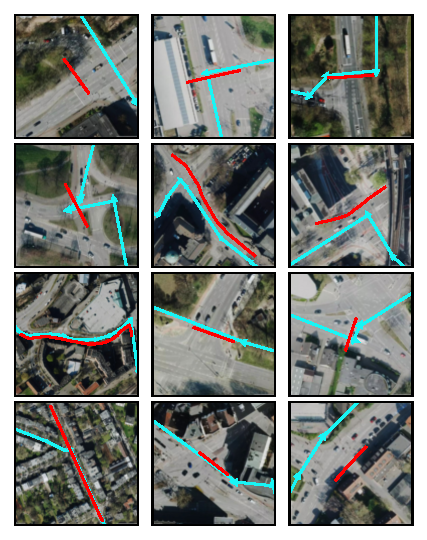
\includegraphics[width=0.46\linewidth]{images/routing-lane-alignment-examples-osm.pdf} & 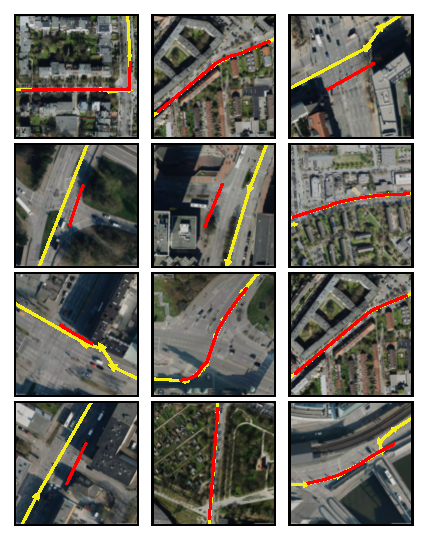
\includegraphics[width=0.46\linewidth]{images/routing-lane-alignment-examples-drn.pdf} \\
\end{tabular}
\caption{.}
\label{fig:}
\end{figure}

\begin{figure}[htbp]
\centering 
\begin{tabular}{cc}
\footnotesize{(a) Redundancy in OSM Ground Truth (2023)} & \footnotesize{(b) Redundancy in DRN Ground Truth (2023)} \\
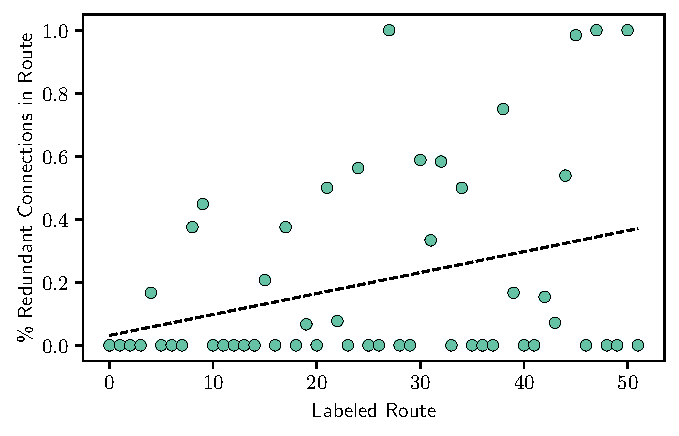
\includegraphics[width=0.45\linewidth]{images/matching-ground-truth-progression-osm.pdf} & 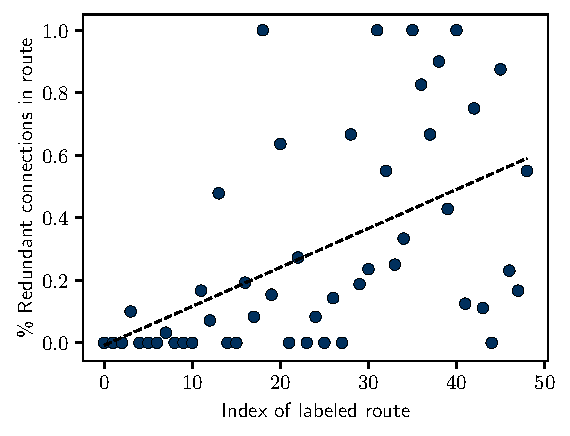
\includegraphics[width=0.45\linewidth]{images/matching-ground-truth-progression-drn.pdf} \\
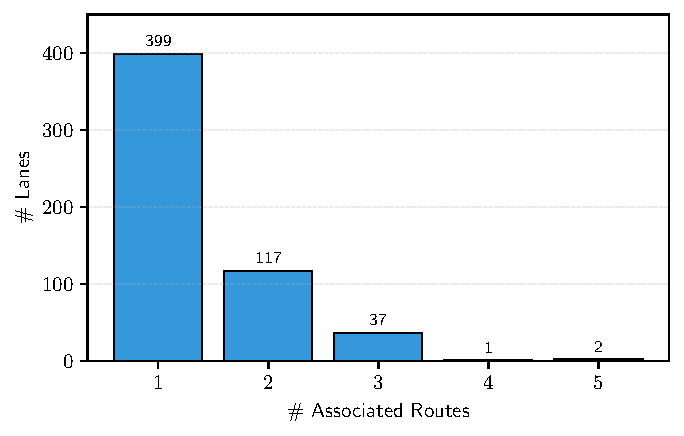
\includegraphics[width=0.45\linewidth]{images/matching-ground-truth-lsas-per-route-osm.pdf} & 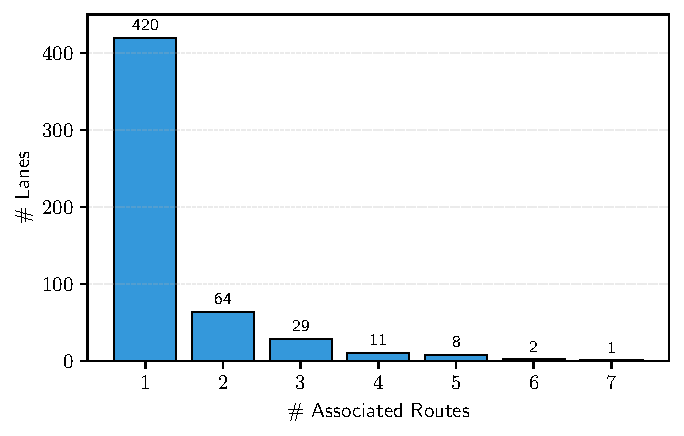
\includegraphics[width=0.45\linewidth]{images/matching-ground-truth-lsas-per-route-drn.pdf} \\
\end{tabular}
\caption{.}
\label{fig:}
\end{figure}

\begin{figure}[htbp]
\centering 
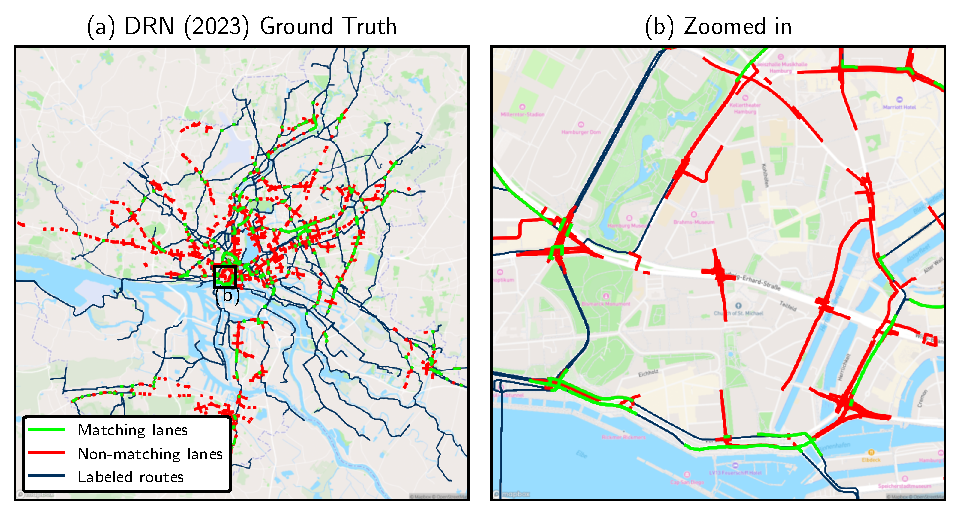
\includegraphics[width=\linewidth]{images/matching-ground-truth-drn.pdf}
\caption{.}
\label{fig:}
\end{figure}

\begin{table}[h]
\caption{Retrained model thresholds on the new routing.}
\begin{tabular}{@{}llllllllll@{}}
\toprule
  \textbf{Ground Truth} & $t_{dist}$ & $t_{bear}$ & $t_{bear\_sum}$ & $t_{inv}$ & $t_{len}$ & $t_{len\_sum}$ & $t_{road\_side}$ &  $t_{perfect\_m.}$ & $t_{overlap}$ \\
  \midrule
  OSM (2022) & 20m & 33° & 79\% & False & 0.99 & 93\% & 59m & 50m & 43\% \\
  OSM (2023) & 19m & 50° & 78\% & False & 0.96 & 77\% & 95m & 46m & 5\% \\
  DRN (2023) & 17m & 27° & 73\% & False & 0.81 & 61\% & 48m & 43m & 59\% \\
\bottomrule
\end{tabular}
\label{tab:hyperparameter-tuning-results-drn}
\end{table}

\begin{table}[h]
\caption{.}
\begin{tabular}{@{}lllllllll@{}}
\toprule
  \textbf{Model} & \textbf{Benchmark} & \textbf{Trained on} & \textbf{TP} & \textbf{FP} & \textbf{FN} & \textbf{Precision} & \textbf{Recall} & \textbf{F1} \\
  \midrule
  Algorithmic & OSM 2022 & OSM 2022 & 920 & 207 & 123 & 82\% & 88\% & 84.8\% \\
  Algorithmic & OSM 2022 & OSM 2023 & 908 & 221 & 135 & 80\% & 87\% & 83.6\% \\
  ML          & OSM 2022 & OSM 2022 & 936 & 57 & 107 & 94\% & 90\% & 91.9\% \\
  \midrule
  Algorithmic & OSM 2023 & OSM 2022 & 615 & 159 & 143 & 79\% & 81\% & 80.3\% \\
  Algorithmic & OSM 2023 & OSM 2023 & 637 & 136 & 121 & 82\% & 84\% & 83.2\% \\
  ML          & OSM 2023 & OSM 2022 & 614 & 52 & 144 & 92\% & 81\% & 86.2\% \\
  \midrule
  Algorithmic & DRN 2023 & DRN 2023 & 655 & 95 & 83 & 87\% & 89\% & 88.0\% \\
  ML          & DRN 2023 & DRN 2023 & 676 & 24 & 62 & 97\% & 92\% & 94.0\% \\
\bottomrule
\end{tabular}
\label{tab:model-scores-drn}
\end{table}

\begin{figure}[htbp]
\centering 
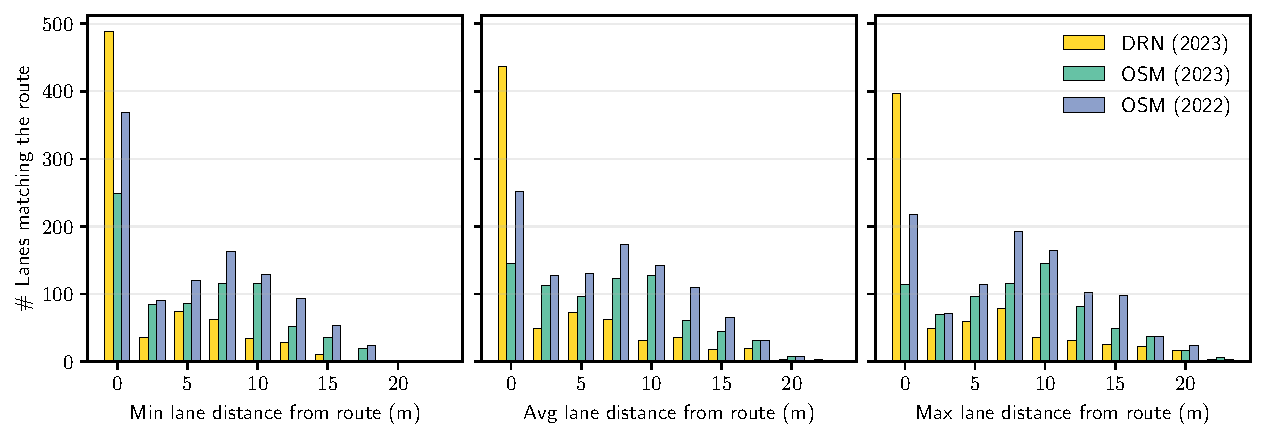
\includegraphics[width=\linewidth]{images/routing-lane-alignment.pdf}
\caption{.}
\label{fig:}
\end{figure}

\begin{figure}[htbp]
\centering 
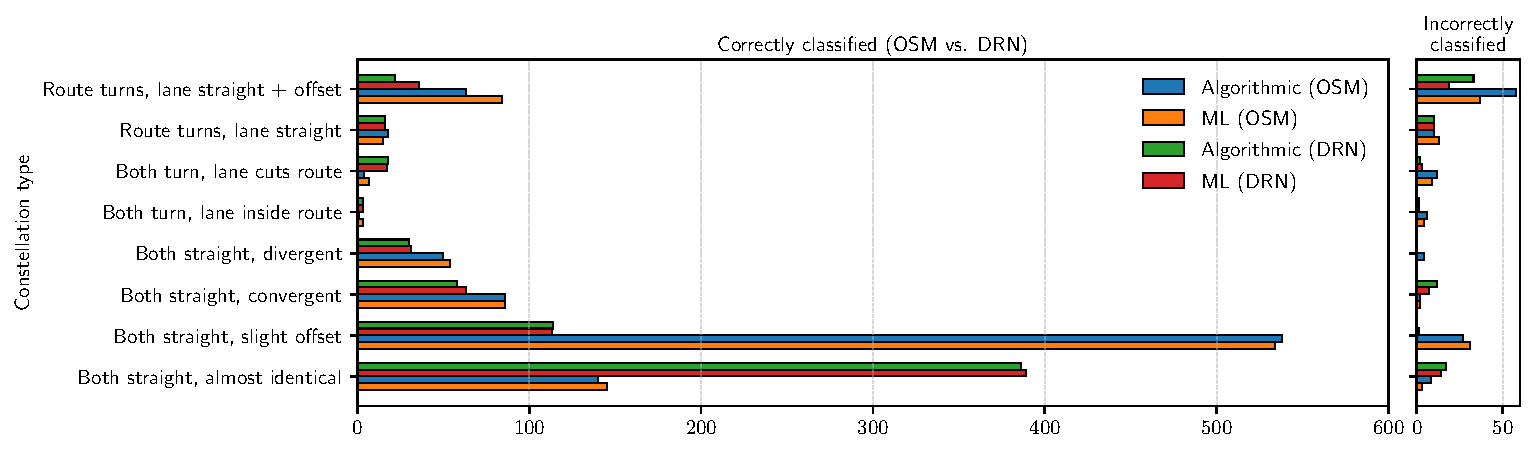
\includegraphics[width=\linewidth]{images/matching-constellations-osm-vs-drn.pdf}
\caption{.}
\label{fig:}
\end{figure}

\begin{figure}[htbp]
\centering 
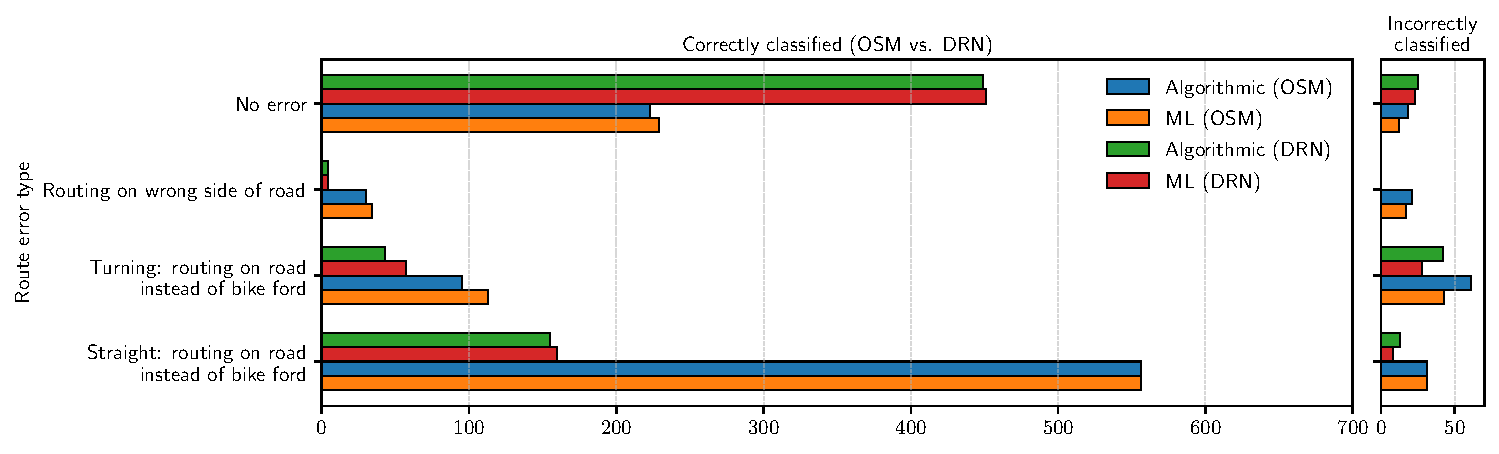
\includegraphics[width=\linewidth]{images/matching-route-errors-osm-vs-drn.pdf}
\caption{.}
\label{fig:}
\end{figure}

\subsection{Comparison with User Trajectories}

- Comparison routing with actual GPS trajectories (map-matching)

- Evaluation rerouting-points, avoided segments

\section{Conclusions}